\documentclass{article}

% Packages for code listing and syntax highlighting
\usepackage{listings}
\usepackage{xcolor}
\usepackage[margin=3cm]{geometry} % Adjust the margin value as desired
\usepackage{setspace}
\usepackage{tikz}
\usepackage{graphicx}
\usepackage{float}
\usepackage{textcomp}
\usepackage{multicol}

% \graphicspath{{!assets}}
\onehalfspacing

% Define the color theme
\definecolor{codebackground}{RGB}{242, 242, 242}
\definecolor{codekeyword}{RGB}{0, 0, 255}
\definecolor{codecomment}{RGB}{63, 127, 95}
\definecolor{codestring}{RGB}{163, 21, 21}

% Code listing style for all languages
\lstdefinestyle{mystyle}{
    backgroundcolor=\color{codebackground},
    basicstyle=\footnotesize\ttfamily,
    keywordstyle=\color{codekeyword}\bfseries,
    commentstyle=\color{codecomment}\itshape,
    stringstyle=\color{codestring},
    numbers=left,
    numberstyle=\tiny\color{codecomment},
    stepnumber=1,
    numbersep=8pt,
    showstringspaces=false,
    breaklines=true,
    frame=single,
    frameround=none,
    framesep=5pt,
    rulecolor=\color{codebackground},
    tabsize=4,
    captionpos=b,
    xleftmargin=15pt,
    xrightmargin=15pt
}

% Set the default style for code listings
\lstset{style=mystyle}

% Additional packages and settings for math typesetting
\usepackage{amsmath}
\usepackage{amssymb}
\usepackage{bm}

% Define your document content
\begin{document}

\title{Modulus-Argument and Exponential Forms of Complex Numbers}
\author{Abyan Majid}
\date{June 17, 2023}
\maketitle

NOTE:
\begin{itemize}
    \item The "Polar" form is also called "Modulus-Argument" form or "Standard Polar" form
    \item The "Exponential" form is also called "Polar exponential" form
\end{itemize}

These are so confusing, so just remember them as "Modulus-Argument" and "Exponential" !

\section{Modulus-argument form}

\fbox{$z=r(\cos\theta + i\sin \theta)$} is the "modulus-argument" form of complex numbers (also known as the "standard polar" form), where:

\begin{itemize}
    \item $z$ is any generic complex number
    \item $r$ is the modulus, $|z|$, of the complex number $z$ (To review, see note "MATH1021/002")
    \item $\theta$ is the argument of the complex number $z$, $arg(z)$, which is specifically the \textbf{angle constructed from the postive real axis to the line of the modulus} $r$. (COMMON MISCONCEPTION: The argument of a complex number is NOT an angle inside of a triangle!)
\end{itemize}

The modulus-argument form is often abbreviated as \fbox{$z=r \text{cis} \phantom{1}\theta$}

\subsection{Making sense of the modulus-argument form}

Given the real part $a$, imaginary part $b$, and modulus $|z|$ of a complex number $z$, we can construct a right-angled triangle where the modulus, $|z|$, is the hypotenuse of the right-angled triangle enclosed by the other two sides $a$ and $b$ (See Figure 1).

\begin{figure}[H]
    \centering
    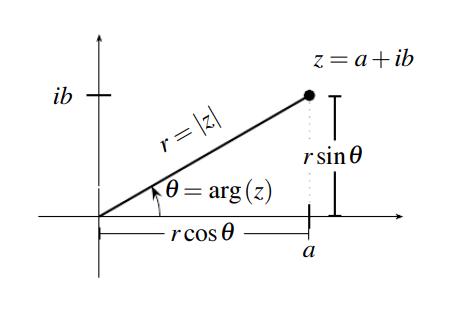
\includegraphics{../../../!assets/MATH1021-003-fig1.png}
    \caption{Right-angled triangle formed by sides $a$, $b$, and $|z|$}
\end{figure}

\subsubsection{Converting real ($a$) and imaginary ($b$) parts into modulus-argument notation}
We can use trig. ratios (sin, cos, tan / SOHCAHTOA) to turn the real part $a$ and imaginary part $b$ into its modulus-argument notations. Given any complex number $z$ and its modulus $|z|$ (which is rewritten as $r$ in the modulus-argument form), we can have the following applications of cos and sin:

\begin{multicols}{2}
    \section*{}
    \vspace{-\baselineskip} % Erases space of section
    $$\cos\theta=\frac{a}{r}$$
    $$a=\cos\theta$$

    \section*{}
    \vspace{-\baselineskip} % Erases space of section
    $$\sin\theta=\frac{b}{r}$$
    $$b=\sin\theta$$
    
\end{multicols}

\subsubsection{How to find the argument $\theta$}

The argument, $\theta$, is NOT an angle inside the triangle formed by $a$, $b$, and $|z|$. It is the angle from the positive real axis until the modulus $|z|$ (See Figure 2).

\begin{figure}[H]
    \centering
    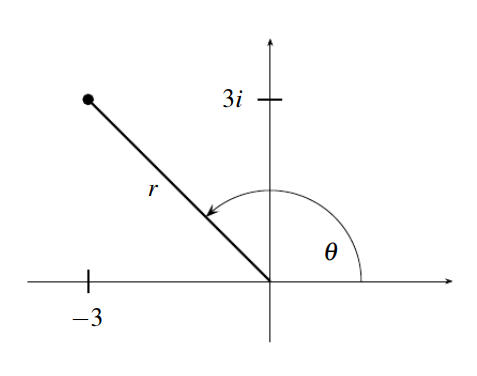
\includegraphics{../../../!assets/MATH1021-003-fig2.png}
    \caption{Argument of a complex number in quadrant 2}
\end{figure}

\noindent So, to identify the argument, simply plot (or imagine plotting)
the complex number on the Argand diagram. It doesn't matter where it's plotted, what you want to do is always go counter-clockwise from the positive real axis until you meet the modulus (or hypotenuse). The angle you'd have drawn then IS the argument.

\vspace{\baselineskip}

\noindent\textbf{ACTUALLY finding the argument just requires applying the "tan" trig. ratio}, where the main intuition is to get the angle of the triangle at the origin, and subtract that from whatever total degree value there is depending on which quadrant the complex number is in.

\begin{center}
    In our Fig. 2 example, we have $z=-3+3i$. Supposing that $\theta_O$ is the angle of the triangle at the origin, we have:
    $$\tan \theta_O=\frac{3}{3}$$
    $$\theta_O=\tan^{-1}\frac{3}{3}=\frac{\pi}{4}$$
    Remember, you don't write $a=-3$, because the sides of a triangle is defined as positive lengths. Now, because $z$ here is in the second quadrant, we can subtract $\theta_O$ from $\pi$ to find the argument $\theta$ in radians.
    $$\theta=arg(z)=\pi-\theta_O$$
    $$\theta=\pi-\frac{\pi}{4}=\frac{3\pi}{4} \text{rad}$$
    So, the argument $\theta$ of the complex number $z=-3+3i$ is \fbox{$\frac{3\pi}{4} \text{rad}$}
\end{center}

\subsection{Principal argument $Arg(z)$}

For any complex number $z$, there is actually infinitely many number of arguments, $arg(z)$, each differing by integer multiples of $2\pi$ radians. This is because $2\pi$ is a full rotation in the Argand diagram. Therefore, if the modulus of any complex number is added or subtracted by $2\pi$, you'd have another argument for the same complex number at the same location.

\begin{center}
    So, the most general form of the argument, $arg(z)$, for any complex number $z$ is: \fbox{$arg(z)=\theta+2k\pi$, $k\in\mathbb{Z}$}
\end{center}

\begin{figure}[H]
    \centering
    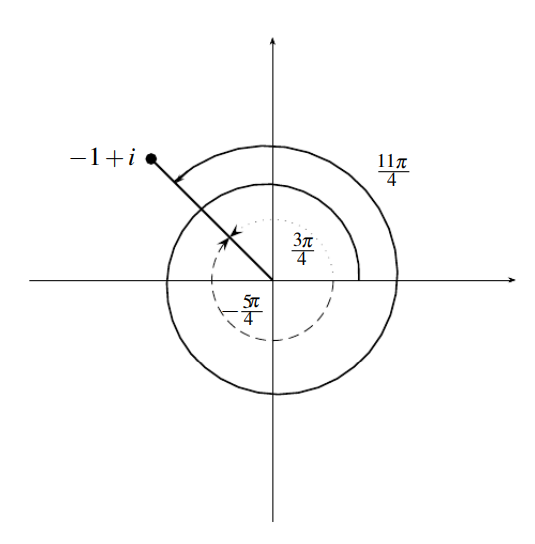
\includegraphics{../../../!assets/MATH1021-003-fig3.png}
    \caption{Infinitely many integer multiples of $2\pi$ for the argument of $-1+i$}
\end{figure}

\begin{center}
    \fbox{The "principal argument", $Arg(z)$, of any complex number $z$ is defined as \fbox{$-\pi<Arg(z)\leq\pi$}.}
\end{center}

\noindent We defined a "principal argument", $Arg(z)$, in order to prevent there being infinitely many arguments for any complex number $z$, such that $Arg(z)$ denotes the argument unique to $z$.

\section{Exponential form}
The exponential form of any complex number $z$ is \fbox{$z=re^{i\theta}$}, where $r$ is the modulus $|z|$, $\theta$ is the argument $arg(z)$, and $e^{i\theta}$ is taken from Euler's formula,
\vspace{-\baselineskip}
\begin{center}
$$e^{i\theta}=\cos\theta + i\sin\theta$$ 
so that,
$$z=r(\cos\theta+i\sin\theta)=re^{i\theta}$$.
\end{center}

\noindent The relationship between the exponential form and the modulus-argument form should be self-explanatory. So, to convert from exponential form to Cartesian form, it's easier to always convert to the modulus-argument form first.

\subsection{Preferably use the exponential form for multiplication and division between two complex numbers!}

The exponential form, $z=re^{i\theta}$, makes multiplication and division between two complex numbers so much easier than if done in the Cartesian or modulus-argument form. But it sucks at addition and subtraction - better rely on the Cartesian form for those instead.

\subsubsection{Multiplication in exponential form}
Multiply the moduli $r_1$ and $r_2$, and add the arguments $\theta_1$ and $\theta_2$ together.

$$z_1 \times z_2 = r_1e^{i\theta_1} \times r_2e^{i\theta_2}$$
$$=r_1r_2e^{i\theta_1+\theta_2}$$

\subsubsection{Division in exponential form}
Divide the moduli $r_1$ and $r_2$, and subtract the arguments, where the divisor and the subtractor comes from the complex number in the denominator.

$$\frac{z_1}{z_2}=\frac{r_1e^{i\theta_1}}{r_2e^{i\theta_2}}$$
$$=(\frac{r_1}{r_2})e^{i(\theta_1-\theta_2)}$$

\end{document}